\chapter{Solution} \label{chap:solution} \minitoc

\section*{}

This chapter describes how the problem presented in Chapter \ref{chap:problem_statement} was solved by stating the solution implemented and the reasons for the choices taken.  \textbf{\textcolor{red}{End with the sections' descriptions}}

\section{Overview}\label{sec:solution_overview}

The goal of this dissertation is to modify Node-RED in order to decentralize its architecture, taking advantage of the capabilities of external devices, no matter how limited they are.

The solution implemented was to use the Node-RED instance to orchestrate the decentralization and send tasks to other devices in the network. The devices make themselves known by announcing their address and capabilities to a registry node running in Node-RED. Consequently, Node-RED assigns nodes to devices and communicates each node's assignment via WiFi. Due to the devices' limitations, they cannot run an instance of Node-RED, so Node-RED needs to convert nodes in Javascript to other language that can be interpreted by these devices. The implemented solution requires a Micropython port and a HTTP server that receives and executes a micropython script created by the Node-RED. This script contains the tasks assigned to a device, translated into micropython. 

After the first deployment of the system, the Node-RED instance manages the state of each device, allowing the system to re-orchestrate if any of the devices becomes unavailable.

\begin{figure}[h]
\centering
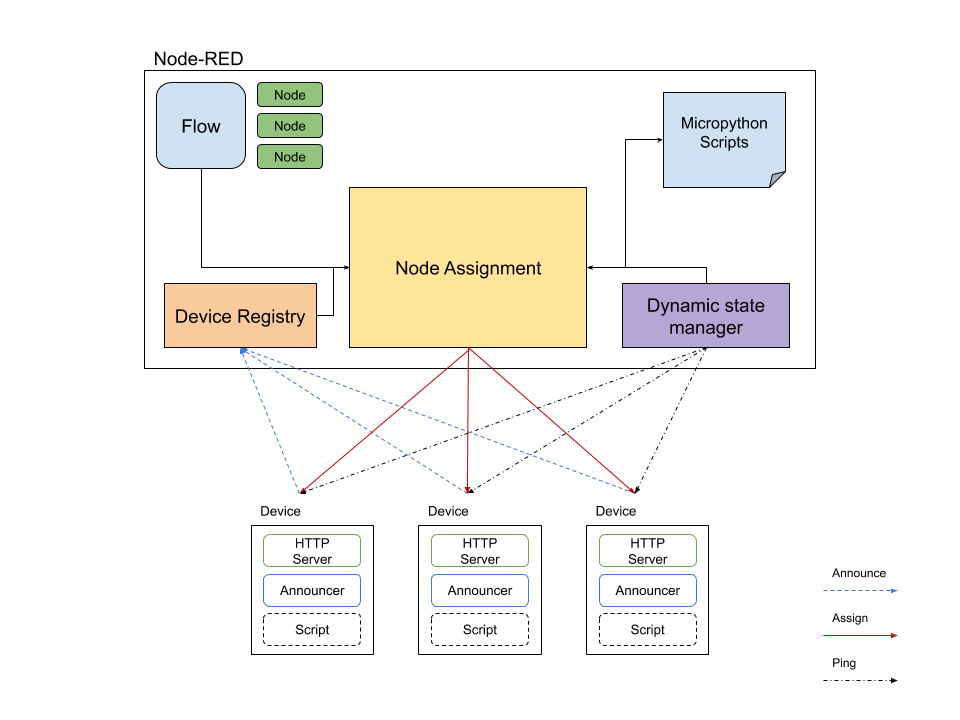
\includegraphics[width=\textwidth]{overview.png}
\caption[Solution's overview]{An overview of the solution}\label{fig:solution_overview}
\end{figure}

\textcolor{blue}{Explain and improve graphic}


\section{Implementation details}\label{sec:implementation_details}

\subsection{Device registry}\label{sec:registry}

When a device becomes available it sends information about itself to a MQTT topic. This information contains the device's IP address, their capabilities and their status - if the device has failed before. In its turn, Node-RED contains a Node called \textit{Registry} that listens to the announcements MQTT topics and saves the devices information. If this node is connected to a orchestrator node, each new device is communicated so that the orchestration can be updated.

When a device has an Out of Memory error, it triggers a fail-safe, where it reboots the HTTP server, stop running any script and restarts all communications. After this action, the device announces itself again but with a flag that indicates that it has failed. This way, Node-RED knows that a device is active but not running any code, and that it possible failed due to too much work. In that case, Node-RED will assign less nodes to the device, reducing the chances of causing another Out of Memory error.

\textcolor{blue}{What is there more to add? Maybe this section is not here, add to other place}

\subsection{Devices setup for decentralization support}\label{sec:devices_decentralization}

The first problem approached in this thesis was finding a way to take advantage of devices with few computational resources, integrating them in a IoT system. The goal was to make these devices execute scripts of code and communicate with other devices, despite their capability limitations. In order to limit the number of type of different devices capable for this aim, only ESP8266 and ESP32 chips were used, since they have connectivity capabilities such as an WiFi chip. In terms of testing, the environment in the devices was replicated in Docker container running the Unix port of micropython.

\subsubsection{Solution overview}

As it was mentioned before in Section \ref{sec:solution_overview}, the devices in the system run a micropython port that allows the execution of scripts written in micropython. This solution is lightweight and extensible. Since these devices need to receive different types of tasks throughout their execution, their firmware includes an HTTP server responsible for receiving scripts of code, saving and executing them. Besides this functionality, it was also implemented an endpoint that returns the state of the device, as well as the announcing mechanism, explained in Section \ref{sec:registry}.

Several micropython libraries were used, more specifically uasyncio and micropython-mqtt. The uasyncio library allowed the implementation of asynchronous operations, critical for the execution of the given script as well as maintaining the HTTP server running and non-blocking.

The firmware also includes a fail-safe mechanism, safeguarding against \textit{out-of-memory} errors that may happen during the lifespan of the device. This mechanism resets all running tasks and recovers the HTTP server and communication channels. This an important feature due to the high probability of these error's occurrence, since the devices have limited memory. 

However, the solution is not perfect and has several limitations, such as:

\begin{itemize}
    \item Support only for mqtt QOS 0 and 1, due to limitations in the MQTT library used. 
    \item ESP8266 memory limitations, where the fail-safe is not possible if the given a script too big.
\end{itemize}

\textcolor{blue}{Maybe add an image explaining the firmware, idk}

\subsection{Node-RED decentralization of computation}\label{sec:node_red_decentralization}

Node-RED is a centralized tool by design, which takes advantage of events to allow communication between nodes in a flow. To implement a decentralized architecture, some changes were made to the Node-RED runtime. These changes consisted in implementing a new way of communication between nodes, detailed in Section \ref{sec:mqtt_support}, as well as implementing specific nodes responsible for the orchestration and registry of devices. \textcolor{blue}{complete later}

\subsubsection{MQTT node communication support}\label{sec:mqtt_support}

Node-RED nodes communicate using events, where a node only communicates with nodes it is wired to. The communication is one way, with the node only sending data to the nodes it is connected to by output. These output wires are used to access the nodes the message must be sent to, and their \texttt{receive()} method is called. This method triggers the event \texttt{emit} which will the caught by a specific method of each node, implementing its own logic.

\textcolor{blue}{Insert code block with example? Or an image explaining?}

This implementation is local and Javascript specific, making it impossible to be used in a decentralized architecture where nodes will be executed outside the Node-RED instance. It was necessary to implement a way of communicating between nodes external to Node-RED that could be supported by low capacity devices. The solution found was MQTT, which fits as a good solution by its low cost and high popularity.

Node entities were changed to support MQTT instead of events, subscribing to topics created at run-time that match the wires between the nodes. Support for sub-flows was also implemented.

\textcolor{blue}{Insert here image that shows a flow with wires and the respective flow with examples of topics}

\subsubsection{Code generation}\label{sec:code_generation}

\textcolor{blue}{Talk about each node code generation, the support for multiple node scripts in one script. Talk about limitation that different nodes on one script, even consecutive nodes, require to communicate with each other by MQTT topics}

As explained above, due to the limitations of the devices used, it was necessary to translate Node-RED nodes, written in Javascript, to micropython code. Along with that, it was also necessary to support multiple nodes in one script, making it necessary to create a generalized script that could fit any type of node.

The implemented solution consists of each node having specific methods related to their functionality and one point of input and output. Since the communication is made by MQTT, as specified in Section \ref{sec:mqtt_support}, the only input a Node can have is in its topics. The same for the output logic. A exception to this is in nodes that are sources, meaning that they generate input and don't receive it. 

The creation the script is made after the assignment of nodes to devices, and each device has its respective script created. The process consists of creating the script with the code of all the assigned nodes and a general code that ties up the script. This general code is responsible for subscribing to all the input topics of all the nodes, stopping the script's processes and forwarding the MQTT messages to the respective node's code.

\textcolor{blue}{Insert Node-RED flow example and the respective micropython script}

\textcolor{red}{Talk about the limitation of communication of two nodes with direct communication being assigned to the same device and still having to communicate to each other via MQTT instead of just calling each other through code.}

\subsubsection{Custom nodes}\label{sec:custom_nodes}

As mentioned before, the orchestration and registry logic are contained in two custom nodes. Besides this two nodes, several others were created in order to test the system and simplify the code generation and others that already existed were altered. 

The nodes created are: (a) If Node, that receives an input and verifies if it complies with all the given rules, returning true or false, (b) And Node, that receives a given number of inputs and verifies if all of them are true or false, returning the corresponding boolean, (c) Temperature-Humidity Node, that read the temperature and humidity from a DHT sensor present in a specific pin, (d) Failure Node, that raises a MemoryError exception, (e) Nothing Node, that simply redirects the received message in its input to its output, and (f) MQTT In and Out Nodes, that subscribe and publish MQTT topics, respectively.

\subsubsection{Computation Decentralization}\label{sec:node_red_computation_decentralization}

The focal point of this dissertation is the decentralization of computation. Given a set of tasks, it must assign them to available devices, ensuring that they will be performed.

To implement this assignment, each device has a set of capabilities, which communicate what the device is capable of doing or accessing, \textit{e.g.} executing micropython code, assessing a DHT sensor, etc. This capabilities are communicated to the orchestrator by the registry, which receives this information by the devices themselves, as is explained in the Section \ref{sec:registry}. 

Besides this, each node has two properties: Predicates and Priorities. Similar to the Kubernetes logic of assigning containers to machines, the predicates dictate constraints that cannot be violated, and priorities are requests that are advisable and recommended but can be violated if impossible to comply. 

The assigning algorithm uses the devices capabilities and each node's predicates and priorities to assign nodes to devices. With a a greedy approach, ir filters the devices that comply with each node's predicates and assigns the one with a higher value of a heuristic. This heuristic takes into account the number of priorities the device can provide, as well as the number of already assigned nodes the device has. The goal is to assign each node to the best possible device, spreading the tasks through all the available devices.

\textcolor{blue}{Insert here assigning algorithm pseudocode}
% node
% bestIndex = 0

% for device in devices:
%     if not all node predicates in device tags: return
%     intersectionIndex = (nº of node priorities in device tags)/(nº node priorities)
    
%     matchIndex = 
%         intersectionIndex * 0.5 + 
%         (1/( nodes assigned to the device) + 1) * 0.4 +
%         (nº of node priorities in device tags/ device tags) * 0.1
    
%     if matchIndex > bestIndex:
%         bestIndex = matchIndex
%         device is the best choice for node

After assigning all nodes to a specific device, a micropython script is generated to each device, as explained in Section \ref{sec:code_generation}. Due to the limitations in memory of the devices, the quantity of nodes assigned to a device may be excessive to its capabilities. In that case, the device will fail-safe and return an error to the assignment request. The orchestrator will receive this information and repeat the process, assigning less nodes to the devices that returned a memory error. If a device does not return any response, the orchestrator will assume that the device is unavailable and not assign any node to it.

\textcolor{blue}{Add an example of an assignment (JSON file) or/and a visual alternative with blocks and labels. With devices with capabilities and the assigned nodes predicates and priorities.}

The process explained above is triggered by four types of events: (1) start of the system, when there is already a defined flow in the configuration, the assignment start after a period of 3 seconds, to give time for the devices to be registered by the registry node; (2) deployment of the entire flow using the Node-RED editor or API; (3) appearance of a new device, with the announcement of it to the registry node; (4) failure or recovery of a device, communicated by the dynamic state management mechanism, detailed in Section \ref{sec:dynamic_state_management}.

\textcolor{blue}{Maybe add an image of the process, with the possible steps that can trigger an announcement, or the flow of the process}

However, due to the use of a greedy algorithm, there are some limitations in the assignment. Besides not resulting in the best possible solution, there is specific situations that can result in the impossibility of complying with the constraints imposed by nodes. For example, given a scenario where the number of devices is small for the quantity of nodes, resulting in the devices being at the limit of their memory capabilities. If there is a node which constraints can only be complied by one device, but that one device already has the maximum number of nodes it can handle, the assignment is not possible.

\textcolor{red}{Falar tmb (?) que o algoritmo não tem em conta o facto de dois nós seguidos ficarem no mesmo dispositivo - isto agora não tem mt impacto pq toda a comunicação é feita por MQTT mas uma possibilidade era 2 nós seguidos ficarem no mesmo dispositivo e comunicarem chamando a função do outro em vez de ser por MQTT}

\subsubsection{Dynamic state management}\label{sec:dynamic_state_management}

After the assignment process, each device is doing their part to allow the system to work as expected. However, given the simplicity of the devices used, such as ESP8266s and ESP32s, they are prone to failures, with possible causes ranging form power loss to faulty hardware, among others.

Due to this limitations, the orchestrator periodically pings the devices in the system, registering any change in their state. If a state is noticed, the orchestrator will repeat the process of assignment taking into account the changes in the device's availability. This detects not only non-availability but also if a device becomes active again after a failure.

\textcolor{blue}{Don't know what to add more}

\subsubsection{Limitations}\label{sec:limitations}

\begin{itemize}
    \item Number of nodes that support micropython code generation is small
    \item Duplicate messages when redeploying the totality of the flow (maybe fixable later)
    \item Re-orchestration only supported when deploying the entire instance (all flows)
    \item Nodes do not stop working when the Node-RED instance is stopped
    \item Script generated does not take into account nodes that communicate directly, forcing all communications through MQTT instead of a node calling the method of another with the output as argument.
    \item Assignment algorithm does not take into account the assignment of sequential nodes in the same device.
\end{itemize}
